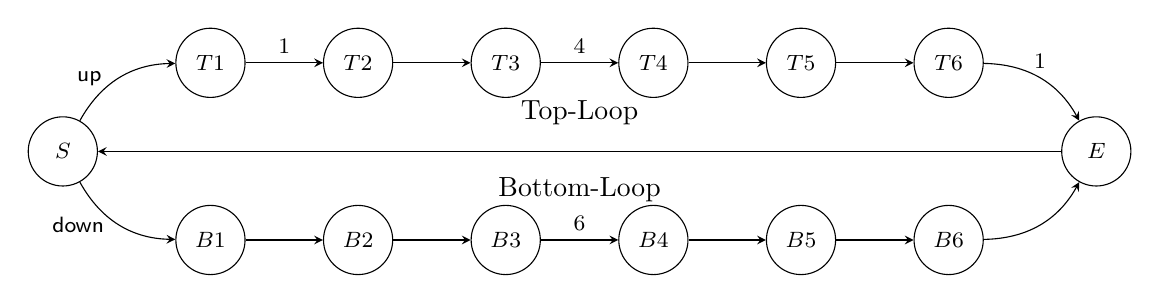
\begin{tikzpicture}[thin, scale=0.75]

  % Nodes
  \draw (-2.5   ,0)  node(S)  [circle,draw,minimum size=25] {\footnotesize \(S\)};
  \draw (0.0  ,1.5)  node(T1) [circle,draw,minimum size=25] {\footnotesize \(T1\)};
  \draw (2.5  ,1.5)  node(T2) [circle,draw,minimum size=25] {\footnotesize \(T2\)};
  \draw (5.0  ,1.5)  node(T3) [circle,draw,minimum size=25] {\footnotesize \(T3\)};
  \draw (7.5  ,1.5)  node(T4) [circle,draw,minimum size=25] {\footnotesize \(T4\)};
  \draw (10.0 ,1.5)  node(T5) [circle,draw,minimum size=25] {\footnotesize \(T5\)};
  \draw (12.5 ,1.5)  node(T6) [circle,draw,minimum size=25] {\footnotesize \(T6\)};
  \draw (0.0  ,-1.5) node(B1) [circle,draw,minimum size=25] {\footnotesize \(B1\)};
  \draw (2.5  ,-1.5) node(B2) [circle,draw,minimum size=25] {\footnotesize \(B2\)};
  \draw (5.0  ,-1.5) node(B3) [circle,draw,minimum size=25] {\footnotesize \(B3\)};
  \draw (7.5  ,-1.5) node(B4) [circle,draw,minimum size=25] {\footnotesize \(B4\)};
  \draw (10.0 ,-1.5) node(B5) [circle,draw,minimum size=25] {\footnotesize \(B5\)};
  \draw (12.5 ,-1.5) node(B6) [circle,draw,minimum size=25] {\footnotesize \(B6\)};
  \draw (15.0 ,0)  node(E) [circle,draw,minimum size=25]    {\footnotesize \(E\)};

  % Edges
  \path[thin, ->, bend left, >=stealth] (S)  edge[above, near start] node[xshift=-3] {\footnotesize \textsf{up}} (T1);
  \path[thin, ->,            >=stealth] (T1) edge[above] node {\footnotesize \(1\) } (T2);
  \path[thin, ->,            >=stealth] (T2) edge[above] node {\footnotesize     } (T3);
  \path[thin, ->,            >=stealth] (T3) edge[above] node {\footnotesize\(4\)} (T4);
  \path[thin, ->,            >=stealth] (T4) edge[above] node {\footnotesize     } (T5);
  \path[thin, ->,            >=stealth] (T5) edge[above] node {\footnotesize     } (T6);
  \path[thin, ->, bend left, >=stealth] (T6) edge[above] node {\footnotesize\(1\)} (E);

  \path[thin, ->,bend right, >=stealth] (S)  edge[below, near start] node[xshift=-7] {\footnotesize \textsf{down} } (B1);
  \path[thin, ->,            >=stealth] (B1) edge[above] node {\footnotesize     } (B2);
  \path[thin, ->,            >=stealth] (B2) edge[above] node {\footnotesize     } (B3);
  \path[thin, ->,            >=stealth] (B3) edge[above] node {\footnotesize\(6\)} (B4);
  \path[thin, ->,            >=stealth] (B4) edge[above] node {\footnotesize     } (B5);
  \path[thin, ->,            >=stealth] (B5) edge[above] node {\footnotesize     } (B6);
  \path[thin, ->,bend right, >=stealth] (B6) edge[above] node {\footnotesize     } (E);

  \path[thin, ->,            >=stealth] (E)  edge[above] node   {\footnotesize} (S);

  
  \draw (6.25,0.65)  node[] { Top-Loop    };
  \draw (6.25,-0.65) node[] { Bottom-Loop };
\end{tikzpicture}

%%% Local Variables:
%%% mode: latex
%%% TeX-master: "../paper"
%%% End:


